
\subsection{Reactions}

\subsubsection{\texttt{ChemicalReaction}}

Nothing particular.

\subsubsection{\texttt{SequenceBinding}}

\paragraph{Binding} Because of the way \texttt{BindingSiteFamily} is implemented, the reaction can easily and efficiently access the binding rate at all times, no matter what reactions have occured previously and how site availability changed in the meantime.

\paragraph{Unbinding} \texttt{SequenceBinding} uses a \texttt{FamilyFilter} (see detailed description of \texttt{BoundChemical}) to filter out all \texttt{BoundUnit}s that are bound to a binding site of the \texttt{BindingSiteFamily} associated with the reaction. \texttt{BoundUnit}s that have bound to sites of a different family or that have moved away from the binding site through \texttt{Translocation} are \emph{not} candidates for unbiding.

\subsubsection{\texttt{Translocation}}

\paragraph{Collisions} For now, \texttt{Translocation} ignores collisions, making its implementation straightforward.

\paragraph{Stalled form}
\begin{itemize}
  \item Translocation enters stalled form if a \texttt{BoundUnit} reached the end of a sequence.
  \item Translocation enters stalled form if a \texttt{BoundUnit} reaches a termination site \emph{after the translocation was completed}. 
\end{itemize}

\subsubsection{\texttt{Loading}}

\paragraph{Handling each polymerase individually} The main challenge with \texttt{Loading} is to maintain the subrates associated with each motif up to date. It needs to maintain a list of all \texttt{BoundUnit}s reading a specifing motif. To this end it uses a \texttt{TemplateFilter} (see detailed implementation of \texttt{BoundChemical}). Every time a \texttt{BoundUnit} becomes of the type of the \texttt{BoundChemical} associated with the reaction, the filter looks what motif defined in the \texttt{LoadingTable} it is currently reading. If the motif could not be found, an \texttt{UNKNOWN TEMPLATE} error message is displayed, the \texttt{BoundUnit} is not recorded in the filter and will not participate in the \texttt{Loading} reaction. The implementation is very similar to that used for \texttt{BindingSiteFamily}~\reffigp{fig:loading}.

\begin{figure}[!h]
  \centering
  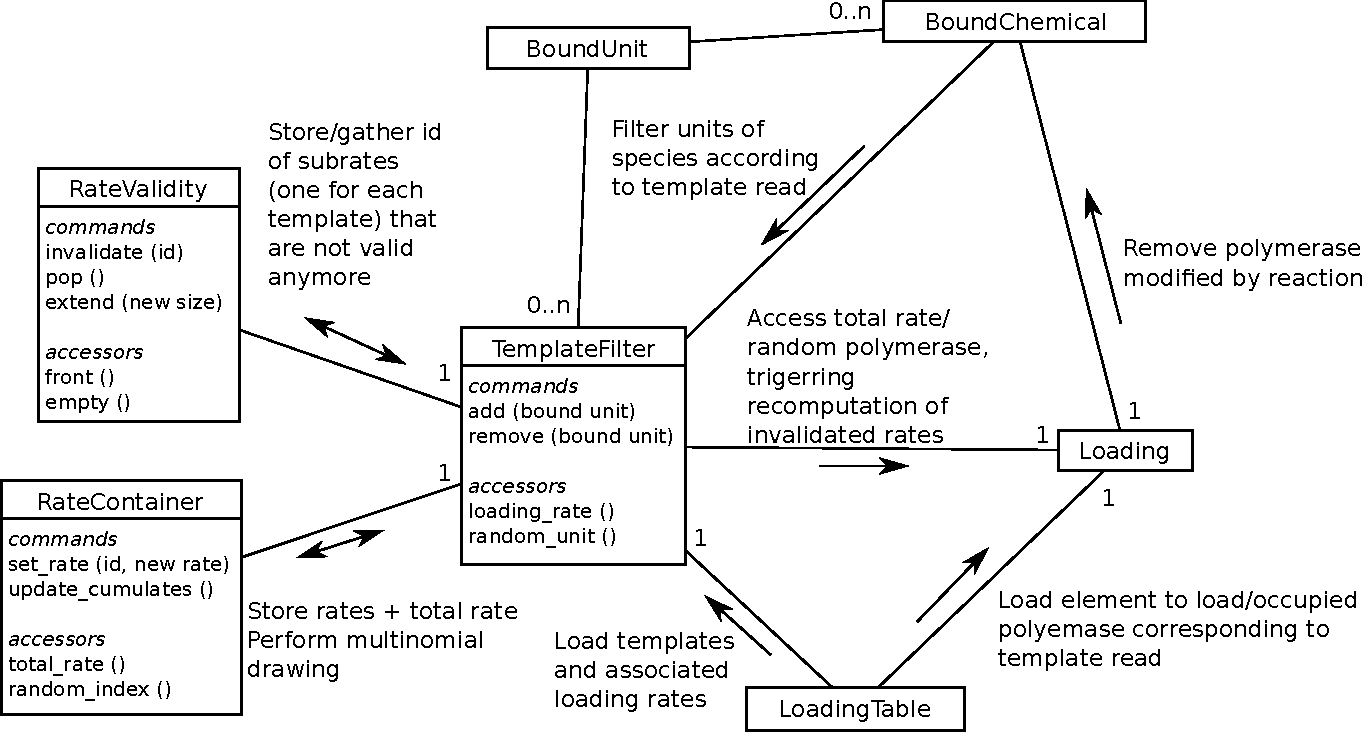
\includegraphics[width=\linewidth]{loading}
  \caption{Schematical view of the pattern used to keep subrates associated with each template up to date in a \texttt{Loading} reaction.}
  \label{fig:loading}
\end{figure}

\paragraph{\texttt{ProductLoading} vs \texttt{DoubleStrandLoading}} There difference between the two processes is rather small. We just added a failure condition in the case of \texttt{DoubleStrandLoading} for convenience. Depending on what reactions are used to synthesize a \texttt{DoubleStrand} it might be possible that a polymerase arrives upon a position that has already been synthesized. In this case, the \texttt{DoubleStrandLoading} fails and the polymerase is replaced by the polymerase in its stalled form.

\subsubsection{\texttt{Release}}

\paragraph{Fail polymerase (unknown product)} When a release is triggered, a \texttt{BoundUnit} from the \texttt{BoundChemical} associated with the \texttt{Release} reaction is randomly chosen. Because the \texttt{BoundUnit} knows its current position and its binding site, it will assume that product it has synthesized starts the \emph{reading frame of the binding site} and ends \emph{at the position directly preceding its current reading frame} (we assume that the polymerase translocates onto a terminating sequence which does not contribute to product synthesis). If the product is found in the \texttt{ProductTable}, everything works normally. 

If the product is not found, we display a \texttt{Unknown Product} error message but keep the simulation alive. The fail polymerase in the reaction enables the user to define a rescue pathway. If the release competes with some other reaction for the original polymerase, the fail polymerase can be the original polymerase itself. If products overlap and the polymerase was stalled due to a termination site of another product, fail polymerase can be a polymerase in a sythesizing step (\textit{e.g.} \texttt{ProductLoading}) so synthesis will resume until the next termination site is reached.
